\documentclass[11pt]{article}

\usepackage[english]{babel}
\usepackage[a4paper,top=2cm,bottom=2cm,left=2.4cm,right=2.4cm]{geometry}
\usepackage{amsmath}
\usepackage{booktabs}
\usepackage{graphicx}
\usepackage{subcaption}
\usepackage{float}
\usepackage{microtype}
\usepackage{xcolor}
\usepackage[colorlinks=true,linkcolor=blue!55!black,citecolor=blue!55!black,urlcolor=blue!55!black]{hyperref}

\newcommand{\code}[1]{\texttt{#1}}
\newcommand{\codelocation}[1]{\par\smallskip\noindent\textbf{Code location:} \path{#1}}

\title{Computer Vision Project\\
\large CNN Classification and Analysis of Fracture Images\\[0.4em]
\normalsize Repository: \href{https://github.com/themoeee/OptML-CNN}{github.com/themoeee/OptML-CNN}}
\author{Moritz Hofer \quad 25-962-689}
\date{}

\begin{document}

\maketitle

\begin{abstract}
This project studies binary fracture classification in $128\times128$ grayscale microscopy images. A compact convolutional neural network (CNN) was trained on the NT dataset and subsequently examined through automated hyperparameter optimization, Gaussian-noise corruption, feature visualization, Grad-CAM, and cross-dataset evaluation. The documented baseline achieved $97.16\%$ test accuracy. Optuna selected a larger $5\times5$ kernel and identified learning rate as the most influential searched parameter. Although the tuned model retained $96.45\%$ accuracy on clean NT test data, its performance approached chance beyond a Gaussian-noise standard deviation of approximately $0.15$. Filter and activation visualizations indicate a progression from local contrast responses to spatially coarser defect-sensitive features, while Grad-CAM localizes the evidence used for an example fracture prediction. Finally, models trained on NT and UT transferred well in both directions. The completed tasks presented here are Tasks 0, 1, 2, 3, and 5.
\end{abstract}

\section{Introduction}

The objective is to classify microscopy images of mechanical test specimens into two approximately balanced classes representing the absence or presence of a fracture. The supplied data contain three experimental categories: ASB (3,741 images), NT (1,407 images), and UT (881 images). Every image is single-channel, has a spatial resolution of $128\times128$, and is normalized to the interval $[0,1]$. For the main NT experiments, the fixed train/validation/test split comprises 844, 281, and 282 images, respectively.

The project follows a staged analysis. Task 0 establishes a reproducible CNN baseline. Task 1 searches its principal optimization and architecture hyperparameters. Task 2 tests whether high clean-data accuracy persists under additive Gaussian noise. Task 3 investigates the learned representation using filters, activation maps, and Grad-CAM. Task 5 finally measures transfer between the NT and UT acquisition domains. Tasks 4 and 6 were not completed and are therefore not presented as results.

\clearpage
\section{Task 0: Baseline CNN Classifier}

\subsection{Approach}

The baseline uses three convolutional layers with 32, 64, and 128 output channels. Each $3\times3$ convolution preserves spatial dimensions through padding and is followed by a ReLU nonlinearity. The first two blocks additionally contain $2\times2$ max pooling, reducing the representation from $128\times128$ to $64\times64$ and then $32\times32$. Adaptive global average pooling maps the final 128 feature maps to a 128-dimensional vector, and a linear layer produces two class logits. The architecture contains 92,930 trainable parameters.

Training minimized cross-entropy using Adam, a learning rate of $10^{-3}$, a batch size of 32, and 150 epochs. Two otherwise identical runs were performed. The first used the original NT training data; the second applied random horizontal flips, rotations of up to $10^\circ$, and translations of up to $10\%$ in each direction. Validation data were used to monitor convergence, and final performance was measured on the held-out NT test split.

\subsection{Results}

\begin{table}[H]
\centering
\caption{Documented baseline results on the held-out NT test set.}
\label{tab:baseline}
\begin{tabular}{lrr}
\toprule
Training setting & Test accuracy & Training time \\
\midrule
Without augmentation & \textbf{97.16\%} & 1 min 54.1 s \\
With augmentation & 96.81\% & 5 min 31.0 s \\
\bottomrule
\end{tabular}
\end{table}

\begin{figure}[H]
\centering
\begin{subfigure}{0.49\linewidth}
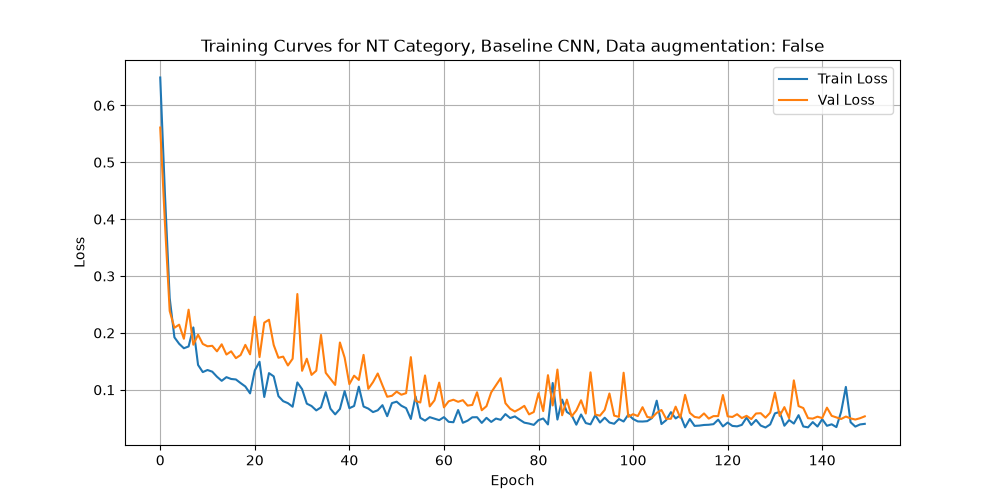
\includegraphics[width=\linewidth]{../../tasks/task_0_baseline_cnn/results/training_curves_NT_baseline_cnn_augFalse.png}
\caption{Without augmentation.}
\end{subfigure}
\hfill
\begin{subfigure}{0.49\linewidth}
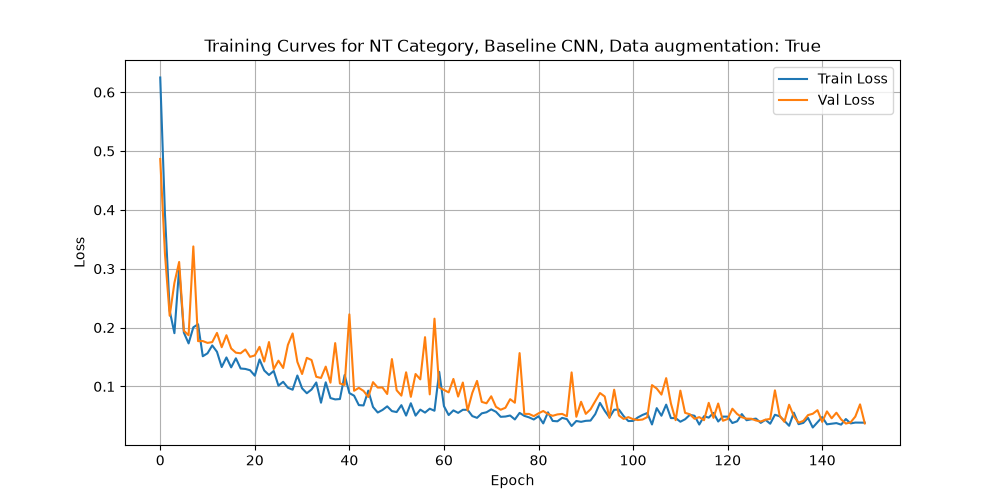
\includegraphics[width=\linewidth]{../../tasks/task_0_baseline_cnn/results/training_curves_NT_baseline_cnn_augTrue.png}
\caption{With augmentation.}
\end{subfigure}
\caption{Training and validation loss of the two baseline runs.}
\label{fig:baseline-curves}
\end{figure}

\subsection{Discussion}

Both configurations classify the NT test set reliably, demonstrating that the comparatively small architecture is sufficient for this binary problem. Augmentation did not improve the documented test accuracy and increased runtime by approximately a factor of 2.9. This result should not be interpreted as evidence that augmentation is generally harmful: the difference is only 0.35 percentage points, each setting was run once, and some geometric transformations may not be exact invariances of the material images. Repeated runs would be needed to separate a systematic effect from random initialization and minibatch-order variation.

The validation curves fluctuate more strongly than the training curves, which is unsurprising for a validation set of only 281 images. Nevertheless, the curves show no persistent divergence that would indicate severe overfitting. The baseline therefore provides a suitable foundation for the subsequent tasks.

\codelocation{tasks/task_0_baseline_cnn/}

\clearpage
\section{Task 1: Hyperparameter Studies and Fine-tuning}

\subsection{Approach}

Optuna~\cite{akiba2019optuna} was used to minimize the best validation cross-entropy reached during training. Each trial trained for 50 epochs. The persistent study database currently contains 75 completed trials; because the search script uses a persistent database with \code{load\_if\_exists=True}, additional executions append trials to the same study. The selected configuration was subsequently retrained for 100 epochs, and the model state with the lowest validation loss was saved.

\begin{table}[H]
\centering
\caption{Optuna search space. Momentum is sampled only for SGD trials.}
\label{tab:search-space}
\begin{tabular}{ll}
\toprule
Hyperparameter & Values or range \\
\midrule
Learning rate & $[10^{-5},10^{-2}]$, logarithmic scale \\
Batch size & $\{8,16,32,64,128\}$ \\
Convolution kernel size & $\{3,5,7\}$ \\
Optimizer & Adam or SGD \\
SGD momentum & $[0,0.95]$ \\
Data augmentation & enabled or disabled \\
\bottomrule
\end{tabular}
\end{table}

\subsection{Results}

The best search-trial validation loss was 0.0171. Its configuration used a learning rate of 0.00658, batch size 8, $5\times5$ kernels, Adam, and data augmentation. Retraining this configuration for 100 epochs produced a saved best validation loss of 0.0391. Evaluation without added noise in Task 2 yielded $96.45\%$ accuracy on the NT test set.

\begin{figure}[H]
\centering
\begin{subfigure}{0.48\linewidth}
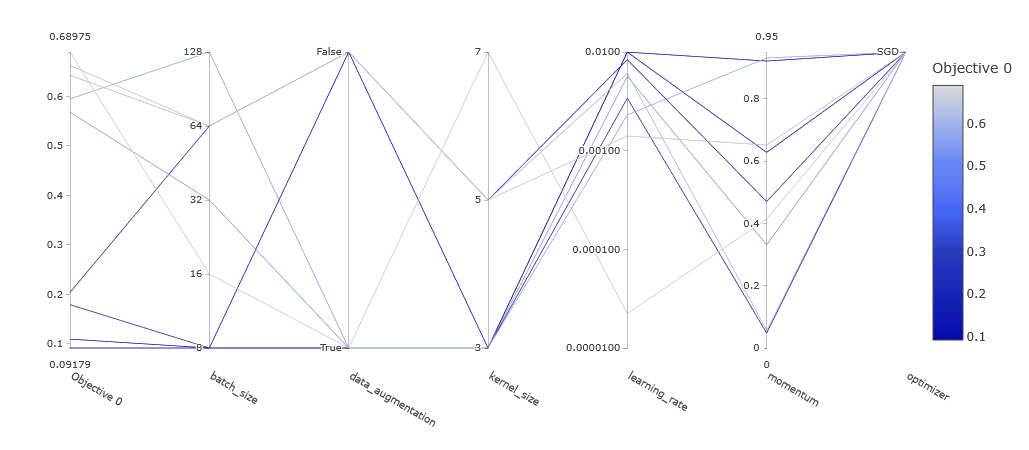
\includegraphics[width=\linewidth]{../../tasks/task_1_hyperparameter/results/task_1_explored_parameters.png}
\caption{Observed objective values across sampled parameters.}
\end{subfigure}
\hfill
\begin{subfigure}{0.48\linewidth}
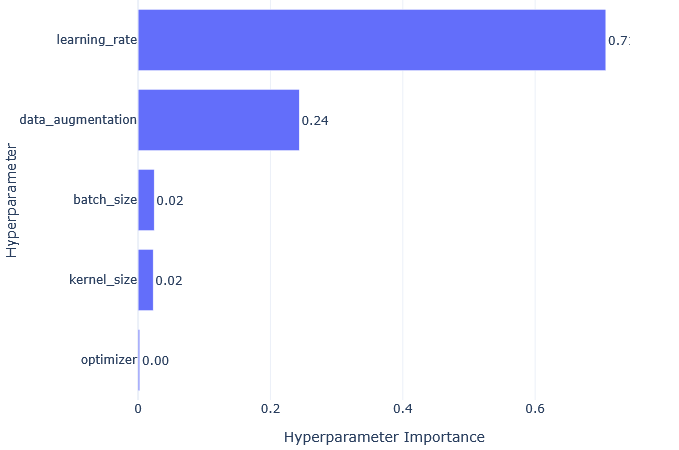
\includegraphics[width=\linewidth]{../../tasks/task_1_hyperparameter/results/task1_hyperparameter_importance_optuna.png}
\caption{Optuna parameter importance.}
\end{subfigure}
\caption{Summary of the completed Optuna study.}
\label{fig:optuna}
\end{figure}

\subsection{Discussion}

Within this finite search space, learning rate explains most of the variation assigned by Optuna's importance estimator (approximately 0.71), followed by augmentation (approximately 0.24). Batch size and kernel size each receive much smaller importance, and optimizer choice contributes little. This ranking is conditional on the selected ranges, trial budget, and 50-epoch objective; it is not a universal statement about CNN training.

The best trial's relatively large learning rate permits rapid optimization within the fixed epoch budget, while the small batch size increases the number of parameter updates per epoch. The difference between the best trial loss and the final retraining loss also illustrates stochastic variation: repeating an identical hyperparameter configuration does not reproduce the same minimum exactly. A stronger final protocol would repeat promising configurations with several seeds and evaluate the test set only after model selection is complete.

\codelocation{tasks/task_1_hyperparameter/}

\clearpage
\section{Task 2: Robustness to Gaussian Noise}

\subsection{Approach}

The tuned NT model from Task 1 was evaluated without retraining after corrupting each test image $x$ according to
\begin{equation}
\widetilde{x}=\operatorname{clip}_{[0,1]}(x+\epsilon),
\qquad \epsilon\sim\mathcal{N}(0,\sigma^2).
\end{equation}
Nine values from $\sigma=0$ to $0.5$ were tested. This measures robustness to a common random corruption rather than adversarial robustness, following the motivation of common-corruption benchmarks such as~\cite{hendrycks2019benchmarking}.

\subsection{Results}

\begin{table}[H]
\centering
\caption{NT test accuracy under additive Gaussian noise.}
\label{tab:noise}
\small
\begin{tabular}{lrrrrrrrrr}
\toprule
$\sigma$ & 0 & .05 & .075 & .10 & .125 & .15 & .20 & .30 & .50 \\
\midrule
Accuracy (\%) & 96.45 & 96.45 & 90.78 & 73.76 & 64.54 & 54.96 & 50.35 & 50.35 & 50.35 \\
\bottomrule
\end{tabular}
\end{table}

\begin{figure}[H]
\centering
\begin{subfigure}{0.59\linewidth}
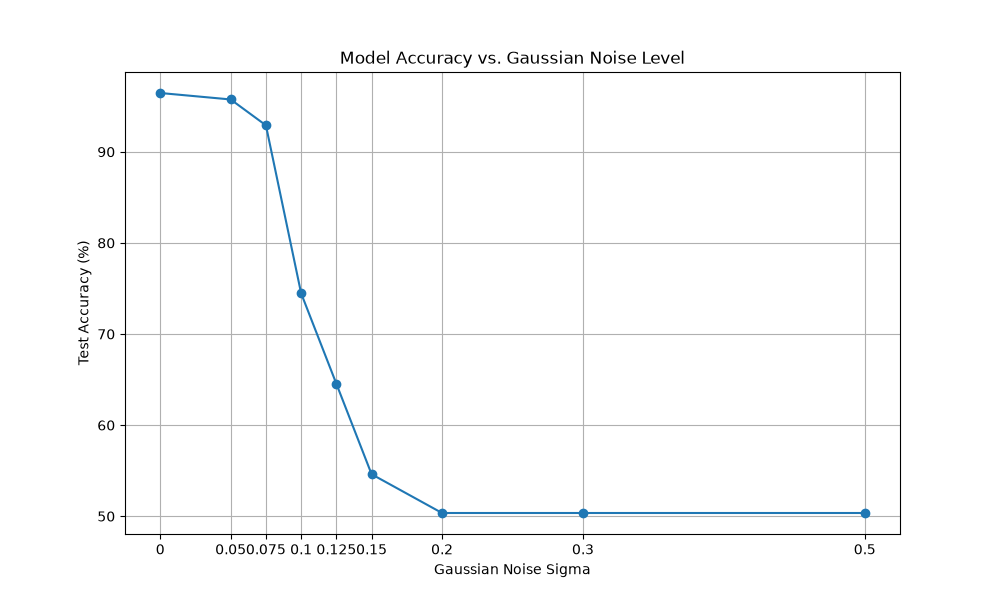
\includegraphics[width=\linewidth]{../../tasks/task_2_robustness/results/accuracy_vs_noise.png}
\caption{Accuracy as a function of noise level.}
\end{subfigure}
\hfill
\begin{subfigure}{0.39\linewidth}
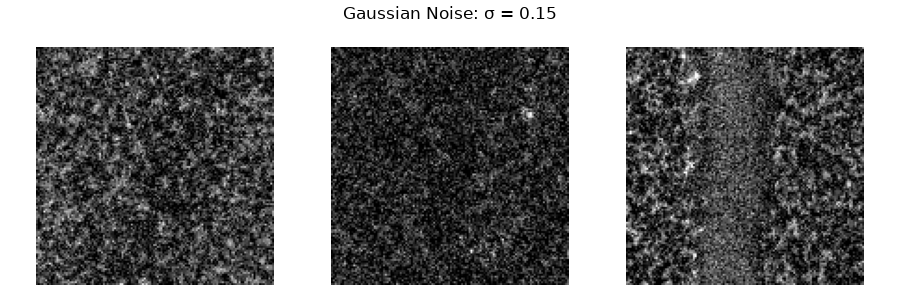
\includegraphics[width=\linewidth]{../../tasks/task_2_robustness/results/sample_images_sigma_0.15.png}
\caption{Examples at $\sigma=0.15$.}
\end{subfigure}
\caption{The model deteriorates rapidly once noise masks the local fracture structure.}
\label{fig:noise}
\end{figure}

\subsection{Discussion}

Accuracy is unchanged at $\sigma=0.05$, but drops by 5.67 percentage points at $\sigma=0.075$ and by a further 17.02 points at $\sigma=0.10$. At $\sigma=0.15$, performance is only 54.96\%; from $\sigma=0.20$ onward it remains at 50.35\%, which equals the majority-class proportion of the almost balanced NT test set. This plateau is consistent with collapse to a single-class prediction.

The qualitative examples explain why a seemingly small numerical standard deviation can be consequential: the task depends on fine local intensity differences, edges, and narrow fracture regions. At moderate noise levels these structures become difficult even for a human observer to distinguish from the material texture. Training with noise, blurred samples, or a mixture of corruptions could improve moderate-noise robustness. However, augmentation cannot recover discriminative information that is no longer visible at severe corruption.

Each image and noise level was sampled once, so the values are single Monte Carlo estimates. Repeating the evaluation with fixed, multiple random seeds and reporting confidence intervals would better quantify uncertainty.

\codelocation{tasks/task_2_robustness/}

\clearpage
\section{Task 3: Feature Visualization and Interpretability}

\subsection{Approach}

Three complementary techniques were applied to the tuned $5\times5$-kernel CNN. First-layer kernels were plotted directly because each consists of one two-dimensional grayscale kernel. Both a global color scale and an individually normalized scale were generated: the former preserves relative weight magnitudes across filters, while the latter makes low-amplitude spatial patterns easier to inspect. Second, post-ReLU activation maps were extracted after each convolutional layer for a correctly classified fracture image. Third, Grad-CAM~\cite{selvaraju2017gradcam} was computed for the final convolutional layer and the predicted class.

The representation changes from 32 maps of size $128\times128$ after the first convolution to 64 maps of size $64\times64$ after the second convolution and 128 maps of size $32\times32$ after the third convolution. Adaptive average pooling subsequently reduces each final map to one scalar before classification.

\subsection{Results}

\begin{figure}[H]
\centering
\begin{subfigure}{0.49\linewidth}
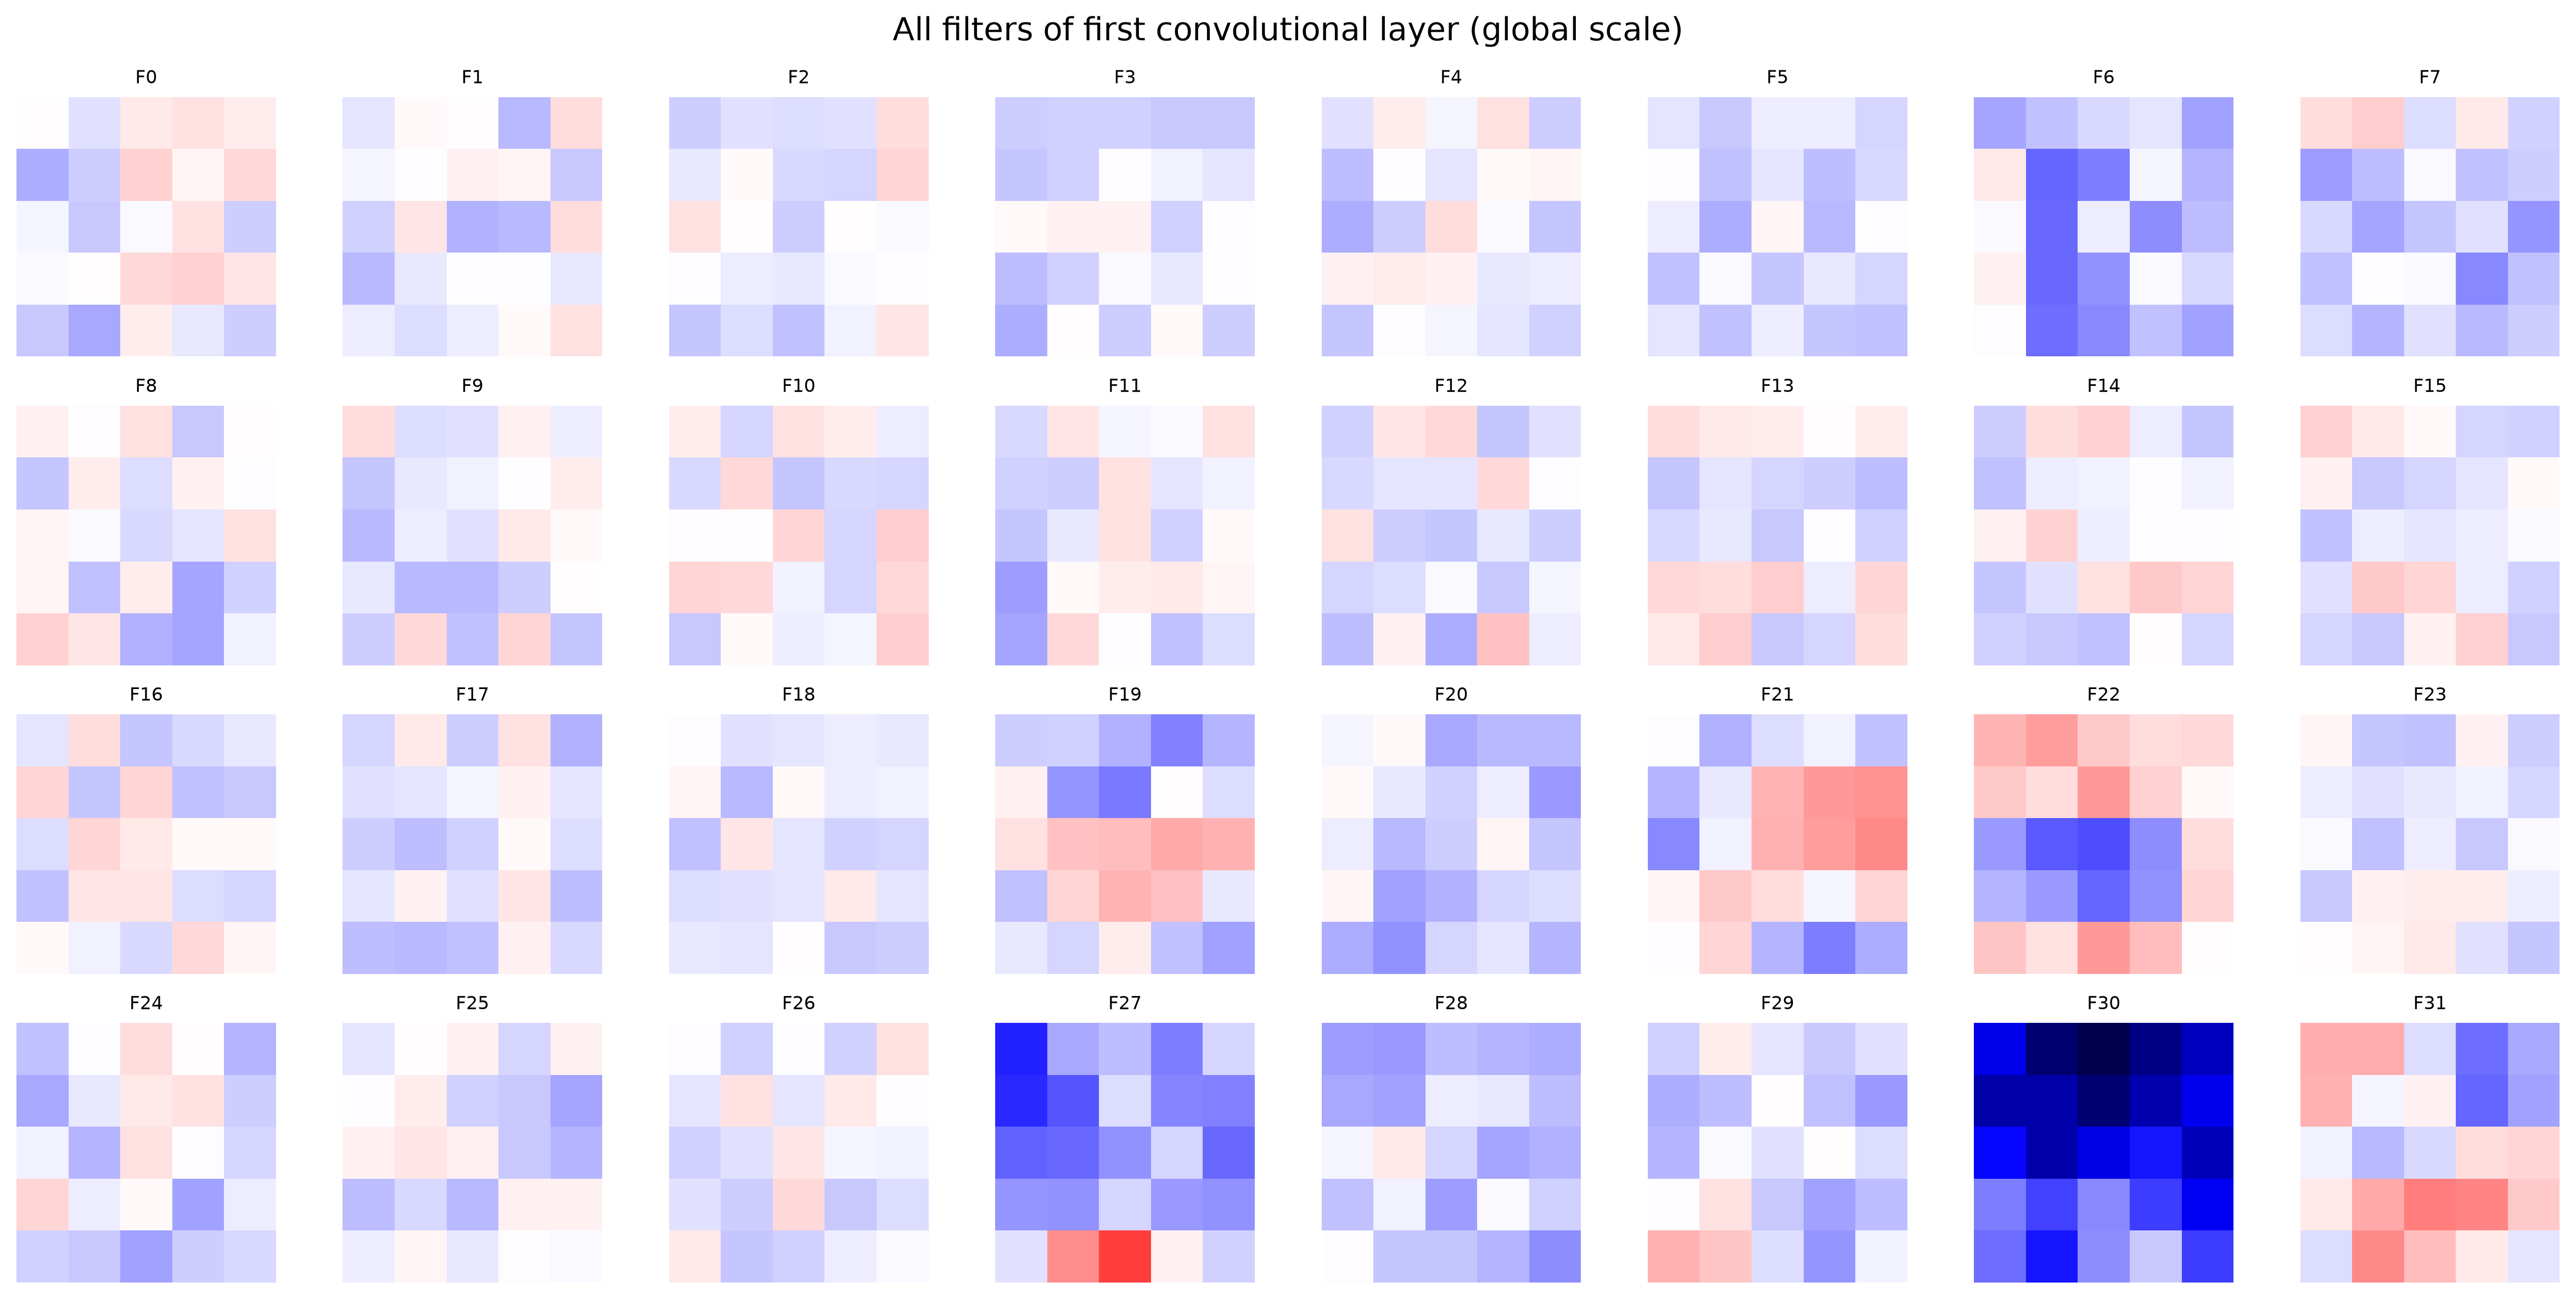
\includegraphics[width=\linewidth]{../../tasks/task_3_interpretability/results/all_filters_conv1_global_scale.png}
\caption{Shared global scale.}
\end{subfigure}
\hfill
\begin{subfigure}{0.49\linewidth}
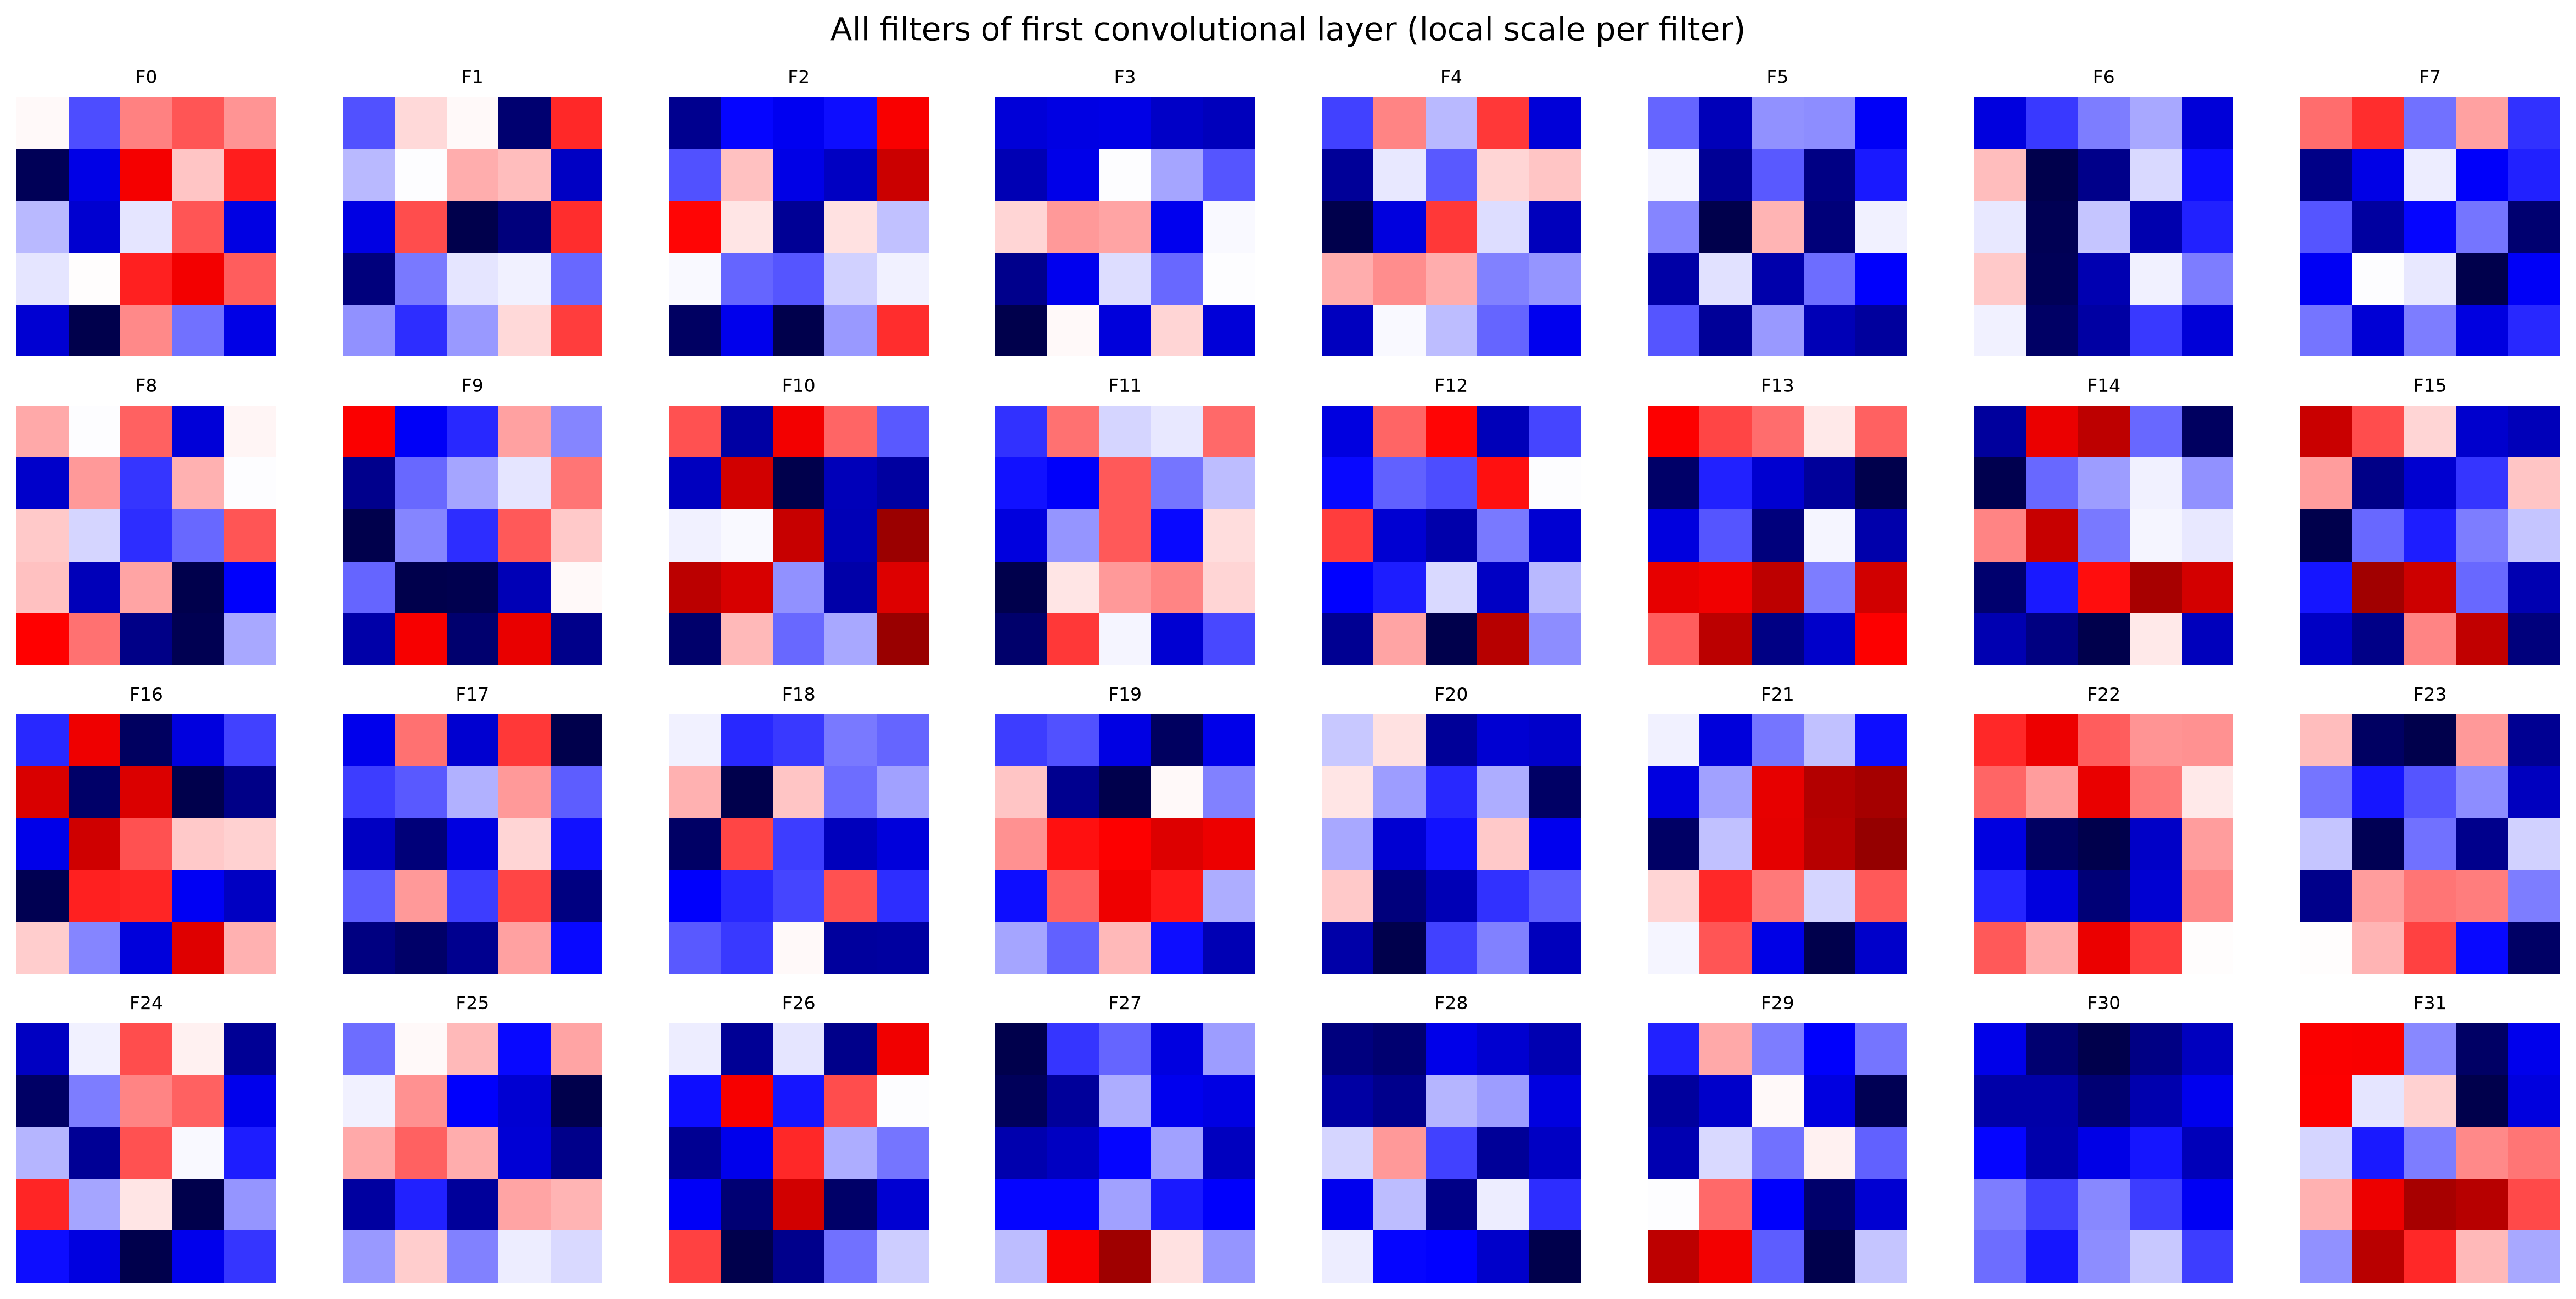
\includegraphics[width=\linewidth]{../../tasks/task_3_interpretability/results/all_filters_conv1_local_scale.png}
\caption{Local scale for each filter.}
\end{subfigure}
\caption{The 32 learned $5\times5$ kernels of the first convolutional layer.}
\label{fig:filters}
\end{figure}

\begin{figure}[H]
\centering

\includegraphics[width=\linewidth]{\detokenize{../../tasks/task_3_interpretability/results/activation_maps_Convolution Layer 1.png}}
\caption{First-layer activations for a correctly classified class-1 sample. Several channels are inactive, while channels such as 21, 22, and 31 respond strongly to local image structure.}
\label{fig:activations-one}
\end{figure}

\begin{figure}[H]
\centering
\begin{subfigure}{0.56\linewidth}

\includegraphics[width=\linewidth]{\detokenize{../../tasks/task_3_interpretability/results/activation_maps_Convolution Layer 3.png}}
\caption{Third-layer activation maps.}
\end{subfigure}
\hfill
\begin{subfigure}{0.42\linewidth}
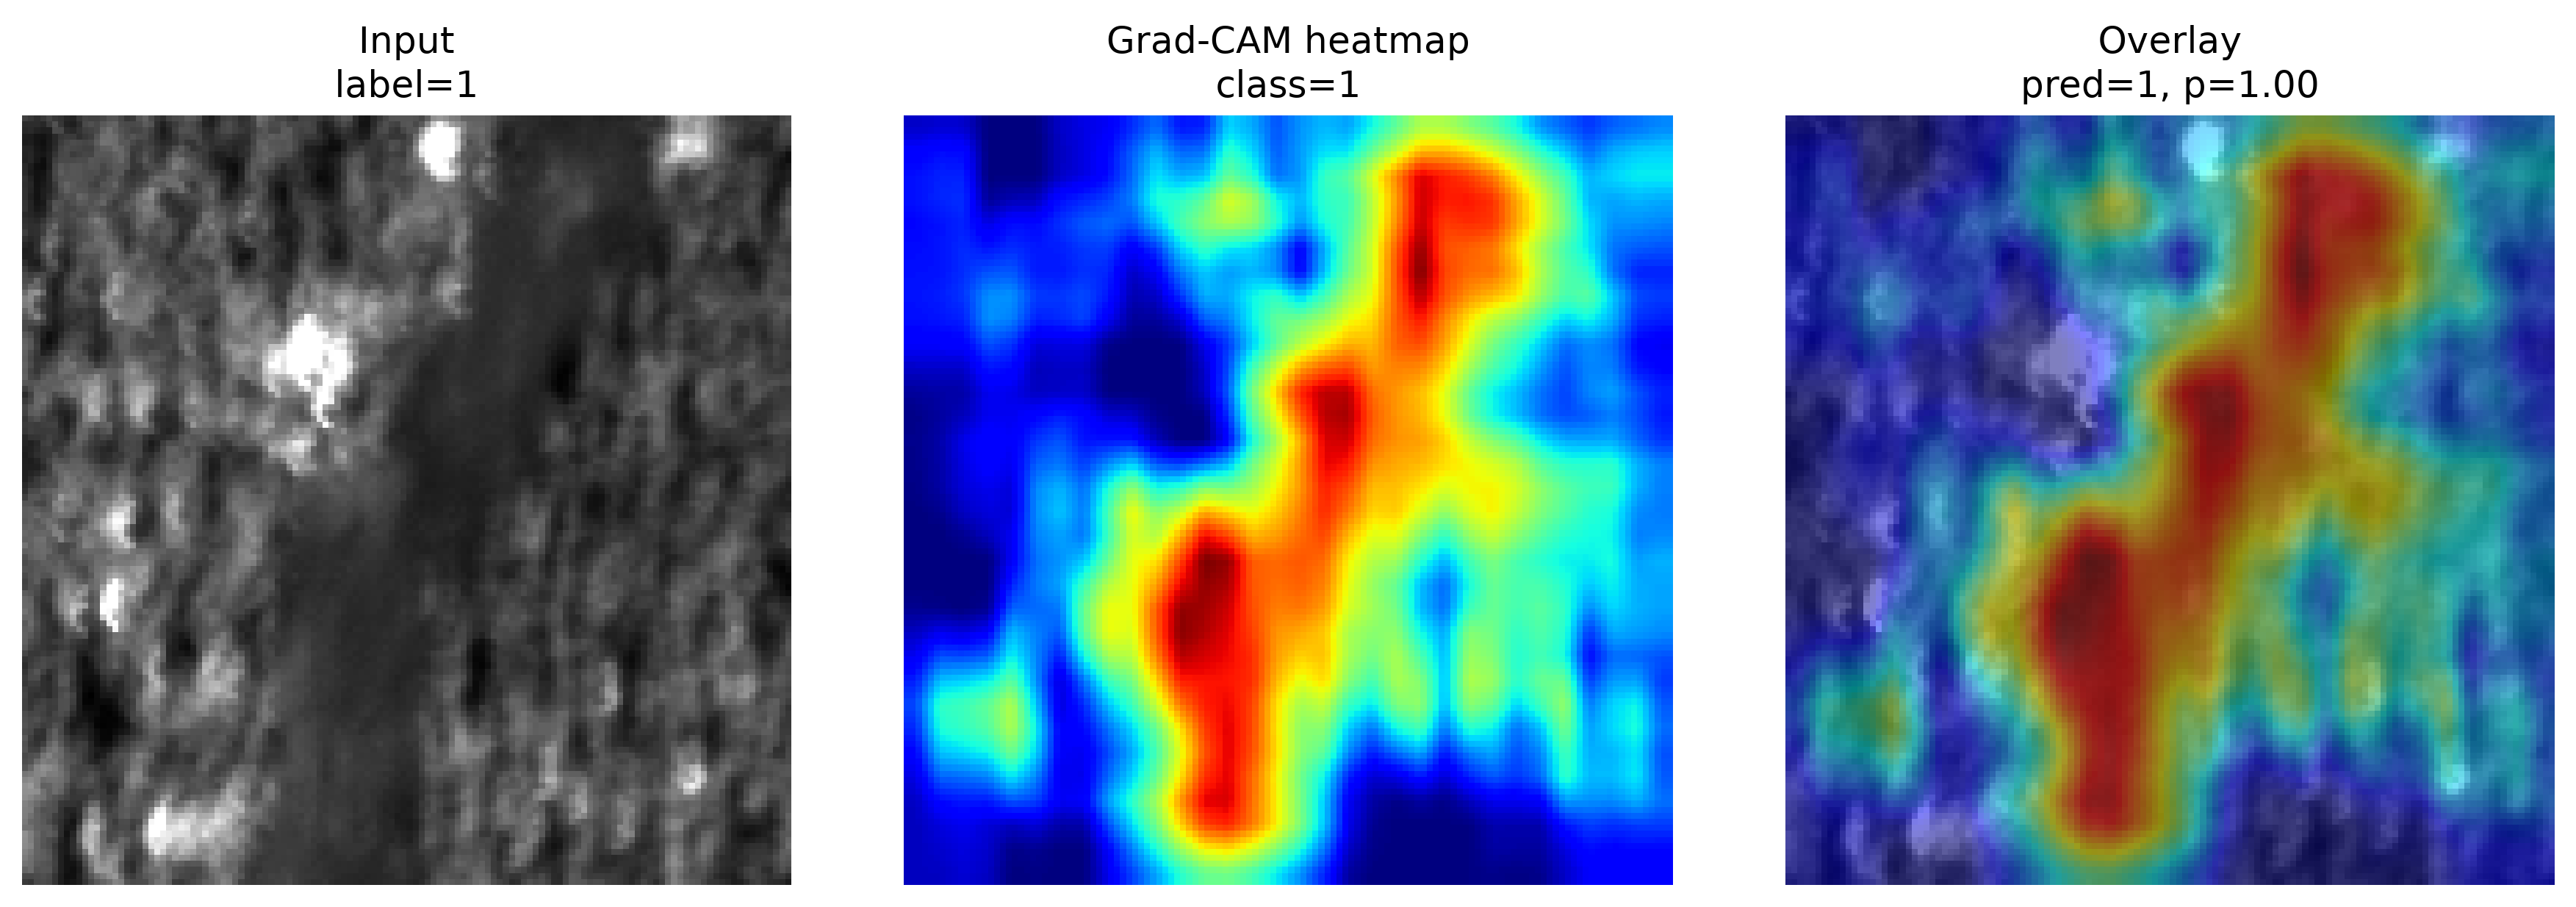
\includegraphics[width=\linewidth]{../../tasks/task_3_interpretability/results/grad_cam_sample_0.png}
\caption{Input, Grad-CAM heatmap, and overlay.}
\end{subfigure}
\caption{Deep activations and Grad-CAM for the same predicted fracture class.}
\label{fig:deep-interpretability}
\end{figure}

\subsection{Discussion}

The globally scaled filter view reveals large differences in learned weight magnitude: filters 27 and 30, for example, have much stronger negative weights than many other filters. The locally scaled view is therefore useful for inspecting weaker patterns, but it must not be used to compare absolute strength. Several kernels resemble local contrast or oriented edge detectors; deeper kernels are not directly interpretable as images because every output filter combines all channels from the preceding layer.

For the selected sample, most early feature maps are suppressed by ReLU, while a smaller set responds to dark regions, boundaries, or textured intact material. The notes identify channels 5, 18, 20, and 30 as dark-region responders and channels 21, 22, and 31 as responding to intact texture. In the second layer, channels 21 and 49 emphasize crack-edge transitions, while channel 48 responds more broadly outside the crack. The third layer contains spatially coarser, more selective responses: several maps activate along the central defect region, whereas others respond to its surroundings. This progression is consistent with a hierarchy from local contrast toward combinations of defect and context features.

The Grad-CAM example places its strongest class-1 evidence along the elongated central structure rather than distributing it uniformly over the image. This supports the interpretation that the prediction uses spatially relevant fracture morphology. It does not, however, prove that every prediction relies on the same cue: the visualization covers one correctly classified example, Grad-CAM is low-resolution, and inactive channels do not necessarily imply that the corresponding learned features are globally unimportant. A larger gallery containing both classes and misclassified samples would strengthen the conclusion.

\codelocation{tasks/task_3_interpretability/}

\clearpage
\section{Task 5: Cross-Dataset Generalization}

\subsection{Approach}

Separate CNNs were trained on NT and UT and evaluated on both held-out test sets without adaptation. The same architecture family and preprocessing were used, so off-diagonal accuracy measures transfer under dataset shift rather than an intentional architecture change. An ASB model was also trained during development, but it reached only 53.67\% on its own test set and approximately chance accuracy elsewhere. Because this indicates an unsuccessful training run or a dataset/pipeline issue, the final generalization matrix excludes ASB rather than presenting its values as meaningful domain-transfer results.

\subsection{Results}

\begin{table}[H]
\centering
\caption{Cross-dataset test accuracy. Rows identify training data; columns identify test data.}
\label{tab:transfer}
\begin{tabular}{lrr}
\toprule
Train $\backslash$ Test & NT & UT \\
\midrule
NT & 96.45\% & \textbf{99.44\%} \\
UT & 94.68\% & 96.61\% \\
\bottomrule
\end{tabular}
\end{table}

\begin{figure}[H]
\centering
\begin{subfigure}{0.43\linewidth}
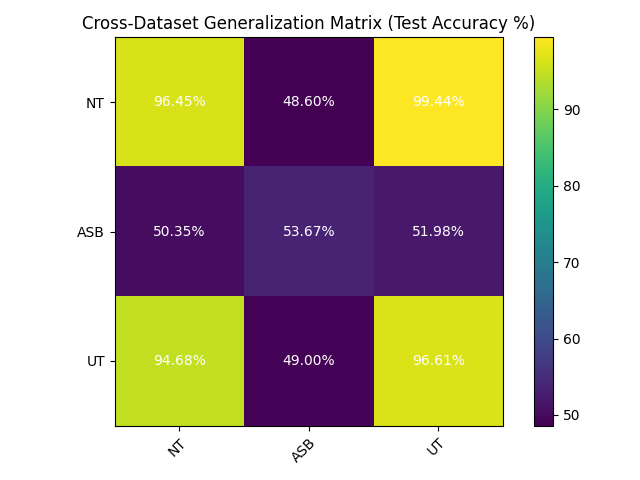
\includegraphics[width=\linewidth]{../../tasks/task_5_cross_dataset/results/cross_generalization_matrix.png}
\caption{NT--UT accuracy matrix.}
\end{subfigure}
\hfill
\begin{subfigure}{0.53\linewidth}
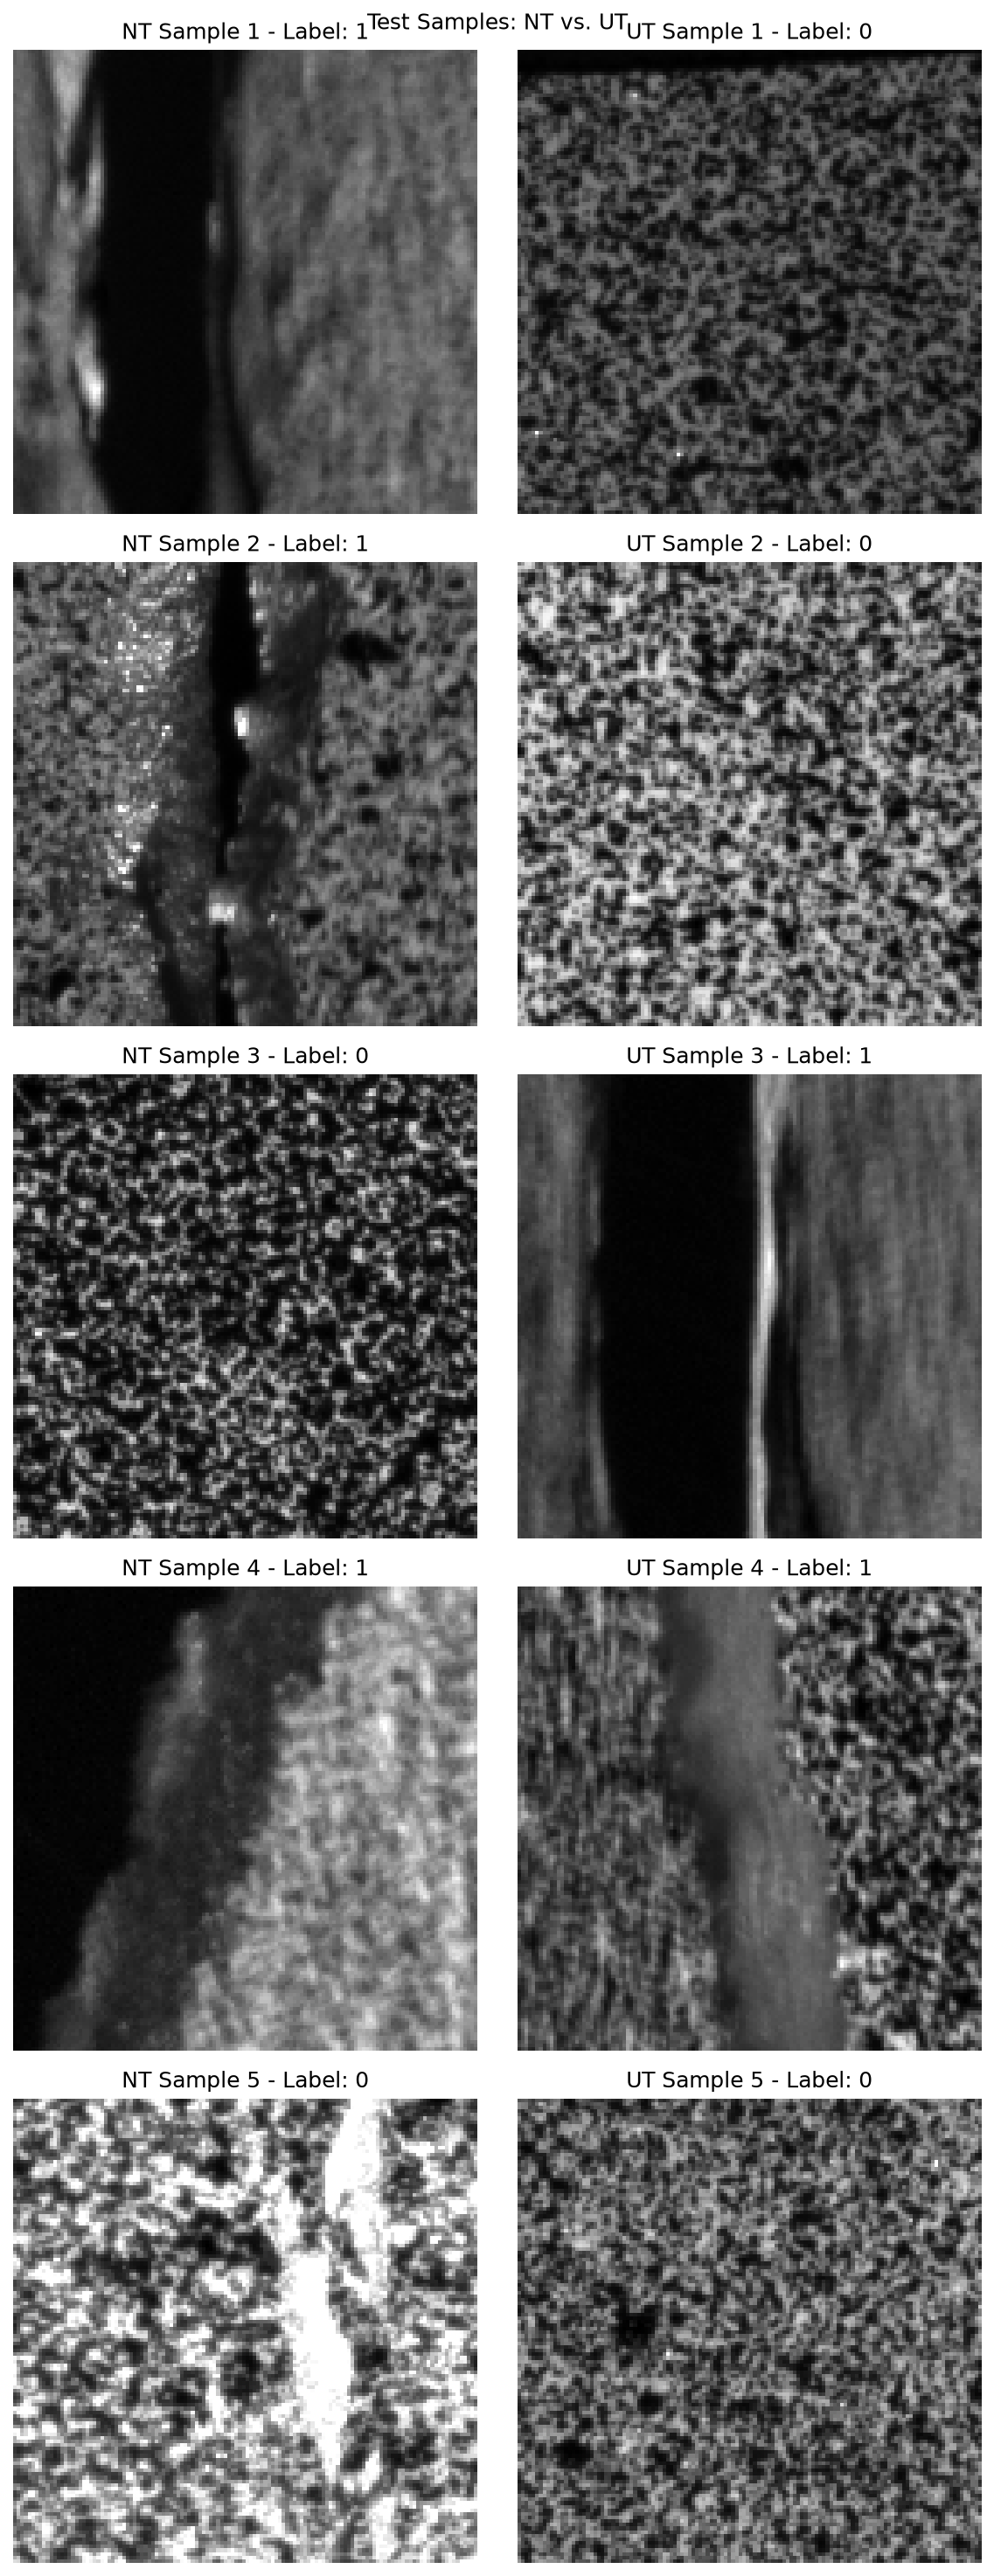
\includegraphics[width=\linewidth]{../../tasks/task_5_cross_dataset/results/sample_images_comparison_NT_UT.png}
\caption{Example NT and UT test images.}
\end{subfigure}
\caption{Cross-dataset evaluation and qualitative comparison of the two domains.}
\label{fig:transfer}
\end{figure}

\subsection{Discussion}

Transfer between NT and UT is strong in both directions. Most notably, the NT-trained model reaches 99.44\% on UT, exceeding both models' within-domain accuracies. This does not imply that cross-domain evaluation is intrinsically easier. A plausible explanation is that the larger NT training set covers the fracture morphologies present in UT, while the UT test split may contain fewer ambiguous examples. Conversely, the UT-trained model reaches 94.68\% on NT; its smaller training set may cover less of the NT variation.

The results suggest that the discriminative features learned for NT and UT are compatible, potentially because both domains share crack-edge and texture cues. Nevertheless, the experiment cannot establish domain invariance. The test sets contain only 282 NT and 177 UT images, and dataset-specific acquisition artifacts could correlate with the labels. The failed ASB run is an additional warning: its labels, normalization, images, training curves, and class-wise predictions should be audited before interpreting ASB transfer.

\codelocation{tasks/task_5_cross_dataset/}

\clearpage
\section{Conclusion}

A compact three-layer CNN is sufficient to classify the NT fracture images with approximately 97\% documented baseline accuracy. Hyperparameter optimization selected Adam with a comparatively high learning rate, a small batch size, $5\times5$ kernels, and augmentation; within the completed Optuna study, learning rate was the dominant parameter. The later analyses show why clean test accuracy alone is incomplete. Performance falls rapidly under moderate Gaussian noise, while interpretability results indicate that the network relies on localized contrast, texture, edge, and defect-region cues. In contrast to its corruption sensitivity, the model transfers strongly between the clean NT and UT domains.

Three limitations recur across the tasks: results are generally based on single training runs, the datasets and test sets are small, and some conclusions rely on qualitative examples. The most valuable next steps are therefore repeated seeded training, uncertainty estimates for the noise experiment, interpretability galleries spanning both classes and failure cases, and a systematic audit of the ASB pipeline. Together these changes would distinguish stable findings from run-specific observations and make the cross-domain conclusions more defensible.

\begin{thebibliography}{9}

\bibitem{akiba2019optuna}
T.~Akiba, S.~Sano, T.~Yanase, T.~Ohta, and M.~Koyama.
\newblock Optuna: A next-generation hyperparameter optimization framework.
\newblock In \emph{Proceedings of the 25th ACM SIGKDD International Conference on Knowledge Discovery \& Data Mining}, 2019.

\bibitem{hendrycks2019benchmarking}
D.~Hendrycks and T.~Dietterich.
\newblock Benchmarking neural network robustness to common corruptions and perturbations.
\newblock In \emph{International Conference on Learning Representations}, 2019.

\bibitem{selvaraju2017gradcam}
R.~R. Selvaraju, M.~Cogswell, A.~Das, R.~Vedantam, D.~Parikh, and D.~Batra.
\newblock Grad-CAM: Visual explanations from deep networks via gradient-based localization.
\newblock In \emph{IEEE International Conference on Computer Vision}, 2017.

\bibitem{muller2021cracks}
A.~M\"uller et al.
\newblock Machine learning classifiers for surface crack detection in fracture experiments.
\newblock 2021.

\end{thebibliography}

\end{document}
